\let\negmedspace\undefined
\let\negthickspace\undefined
\documentclass[journal,12pt,twocolumn]{IEEEtran}
\usepackage{cite}
\usepackage{amsmath,amssymb,amsfonts,amsthm}
\usepackage{algorithmic}
\usepackage{graphicx}
\usepackage{textcomp}
\usepackage{xcolor}
\usepackage{txfonts}
\usepackage{listings}
\usepackage{enumitem}
\usepackage{mathtools}
\usepackage{gensymb}
\usepackage{comment}
\usepackage[breaklinks=true]{hyperref}
\usepackage{tkz-euclide} 
\usepackage{listings}
\usepackage{gvv}                                        
\def\inputGnumericTable{}                                 
\usepackage[latin1]{inputenc}                                
\usepackage{color}                                            
\usepackage{array}                                            
\usepackage{longtable}                                       
\usepackage{calc}                                             
\usepackage{multirow}                                         
\usepackage{hhline}                                           
\usepackage{ifthen}                                           
\usepackage{lscape}
\setlength{\arrayrulewidth}{0.5mm}
\setlength{\tabcolsep}{18pt}
\renewcommand{\arraystretch}{1.5}

\newtheorem{theorem}{Theorem}[section]
\newtheorem{problem}{Problem}
\newtheorem{proposition}{Proposition}[section]
\newtheorem{lemma}{Lemma}[section]
\newtheorem{corollary}[theorem]{Corollary}
\newtheorem{example}{Example}[section]
\newtheorem{definition}[problem]{Definition}
\newcommand{\BEQA}{\begin{eqnarray}}
\newcommand{\EEQA}{\end{eqnarray}}
\newcommand{\define}{\stackrel{\triangle}{=}}
\theoremstyle{remark}
\newtheorem{rem}{Remark}
\begin{document}


\title{Waves(20) 11.15}
\author{EE23BTECH11051-Rajnil Malviya}
\date{January 2024}



\maketitle

\subsection*{\textbf{Question :-}}
A train, standing at the outer signal of a railway station blows a whistle of frequency
400 Hz in still air. (i) What is the frequency of the whistle for a platform observer
when the train (a) approaches the platform with a speed of $10 ms^{-1} $, (b) recedes
from the platform with a speed of $10 ms^{-1} $? (ii) What is the speed of sound in each
case ? The speed of sound in still air can be taken as $340 ms^{-1} $.

\bigskip
Solution :-\\
           frequency of whistle, $F = 400 Hz$\\
speed of sound in air, $a= 340  ms^{-1} $\\
speed of train, $u= 10 ms^{-1} $\\

(i)  a. When the train approaches the platform (i.e., the observer at rest),
\bigskip

$F'_a $ is frequency observed by observer when train is approaching platform ,\\

$$F'_a=F\times\frac{a}{a-u}$$

$$F'_a=400\times\frac{340}{340-10}$$

$$F'_a=412.1212$$
\bigskip

b. When the train recedes the platform (i.e., the observer at rest),
\bigskip

$F'_a $ is frequency observed by observer when train is receding platform,\\
$$F'_r=F\times\frac{a}{a+u}$$

$$F'_r=400\times\frac{340}{340+10}$$

$$F'_r=388.5714$$
\bigskip

(ii) The speed of sound in each will be same.It is $340  ms^{-1}$ in each case.\\

\bigskip

\subsection*{\textbf{Equation of Sound Wave :-}}
Sound Wave is transmission of energy ; sound wave depends on many parameters . A general equation of sound wave is shown below 
$$y(t) = Asin( 2 \pi ft + \phi ) $$  
\textit{y(t) is instantaneous 
displacement of wave at time t;}$$\textit{A is amplitude of wave;}$$$$f\;is\; frequency\; of\; wave;$$
$$t \;is\; time;$$$$\phi \; is \; phase \; angle;$$
\bigskip



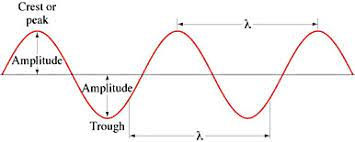
\includegraphics[width=0.45\textwidth]{waves.jpeg}\\
$$\lambda \;is\; wavelength\; of\; wave;$$$$crest \;is\; peak(highest\; point) \;of\; wave;$$$$trough\; is\; dip(lowest\; point) \;of\; wave;$$\\
$$2\pi \;f = \omega;$$
$$\omega \;is\; called \;angular\; frequency;$$
if this is replaced in above equation ; so it reduced to
$$y(t) = Asin(\omega t + \phi ) $$  
\newpage
On comparing above equation with our problem , equation for different cases are given\\\\
$equation \;of\; sound\; wave\; when\; whistle\; is\; blown\; by$
\textit{train is}
$$y(t) = Asin( 2 \pi \times400\times t + \phi ) $$ 
\;\;\;\;\;\;\;\;\;\;\;\;\;\;\;\;\;\;\;\;for this case $f\;=\;400Hz$\\\\
$equation \;of\; sound\; wave\; observed\; by\; observer\;when\\ \;train\;is\; approaching\; observer\;$
$$y(t) = Asin( 2 \pi \times412.1212\times t + \phi ) $$ 
\;\;\;\;\;\;\;\;\;\;\;\;\;\;\;\;\;\;\;\;for this case $f\;=\;412.1212Hz$\\\\
$equation \;of\; sound\; wave\; observed\; by\; observer\;when\\ \;train\;is\; receding\; observer\;$
$$y(t) = Asin( 2 \pi \times388.5714\times t + \phi ) $$ 
\;\;\;\;\;\;\;\;\;\;\;\;\;\;\;\;\;\;\;\;for this case $f \;\;= \;\;388.5714Hz$\\
\subsection*{\textbf{Doppler Effect for Sound Waves :-}}
Doppler effect for sound wave refers to change in frequency or pitch of sound wave observed by an observer when there is a relative motion between observer and source .\\\\

    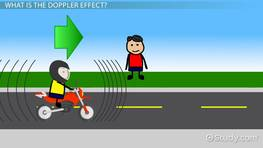
\includegraphics[width=1\linewidth]{doppler.jpg}\\\\

\subsection*{\textbf{Derivation \;of \;Doppler :-}}
To derive Doppler , we can write equation of sound as shown
$$f = \frac{v}{\lambda}$$
$$y(t) = Asin( 2 \pi \frac{v}{\lambda}t + \phi ) $$  
$$v \;is\; speed\; of\; sound\; in\; that\; medium$$
Now consider the relative motion in which source is moving towards observer , in that case effective wavelength $\lambda'$ observed by observer will be compressed ,
$$\lambda' = \lambda - v_o T$$
$$v_o \;is\; relative\; velocity\; of\; observer$$
T is time period(time taken by source wave to complete one revolution)
and effective frequency \textit{f}' observed by observer will be
$$f' = \frac{v}{\lambda'}$$
on substituting values from above we get
$$f' = \frac{v}{\lambda- v_o T}$$
$$f' = \frac{v f}{f(\lambda- v_o T)}$$
we know ,
$$T = \frac{1}{f}$$
$$f' = \frac{v f}{v- v_o }$$
\bigskip
Similarly , if source is receding from observer than $\lambda, $will be increased
$$\lambda' = \lambda + v_o T$$
on substituting this , we get
$$f' = \frac{v}{\lambda+v_o T}$$
$$f' = \frac{v f}{f(\lambda+v_o T)}$$
$$f' = \frac{v f}{v+ v_o }$$
Above equations are suggesting , if source approaches observer or observer approaches source than frequency will increase and if they recedes than frequency will decrease .\\\\
\textit{Doppler effect depends on relative velocity }, so we are providing a table in which different frequencies are given depending on situation .
\newpage

    \begin{table}[h]
        \setlength{\arrayrulewidth}{0.5mm}
\setlength{\tabcolsep}{18pt}
\renewcommand{\arraystretch}{1.5}


\begin{tabular}{ |p{2cm}|p{2cm}p{2cm}p{3cm}|p{1}p{1}}
    \hline
    \multicolumn{4}{|c|}{frequencies observed in Different cases} \\
    \hline
    Doppler Shift &Stationary Observer &Observer moving towards Source &Observer moving away from Source\\
    Stationary Source & $$f' = f$$& $$f' = \frac{(v+v_o) f}{v}$$&$$f' = \frac{(v-v_o) f}{v}$$\\
    Source moving towards Observer &$$f' = \frac{v f}{v-v_s }$$&$$f' = \frac{(v+v_o) f}{v- v_s }$$&$$f' = \frac{(v-v_o) f}{v- v_S }$$\\
    Source moving away from Observer&$$f' = \frac{v f}{v+ v_s }$$&$$f' = \frac{(v+v_o) f}{v+ v_s }$$&$$f' = \frac{(v-v_o) f}{v+ v_s }$$\\
    \hline
    \end{tabular}

    \end{table}

   $v_s\; is\; velocity\; of\; Source\; velocity\; of\; Source\; and\; Observer\; are\; measured\; from\; same\; frame\; of \;reference .$
    


\end{document}
